\section{Introduction}
Web-scale visual data provides massive amount of information while requiring more complex models to take this advantage, therefore, whether we can apply computer vision techniques efficiently enough becomes a bottleneck question.
Robotics is a typical area in need of near real-time performance. Unmanned Aerial Vehicles (UAVs), as a type of the autonomous robotics systems, are increasingly interesting to researchers in recent years. 
They are widely used in applications including reconnaissance and surveillance, search-and-rescue, and infrastructure inspection ~\cite{c1,c3,c5}.
Visual object detection is an important component of such UAV applications.
Moreover, it's also very challenging because of noisy image quality with complex scene and most importantly, the conflict of the near real-time performance requirement and the relatively long running time of advanced object recognition techniques.
Solving this problem not only improves the computer vision component on robotics systems, but also extend the object recognition models based on very large dataset to near real-time applications.

Object recognition performance is rapidly improving mostly based on Deep Learning techniques with Convolutional Neural Networks ~\cite{c13,c14,c15}.
These deep models are trained with very large datasets and are typically consist of millions or billions of parameters. 
These computational demanding techniques require the support of hardware including gigabytes of memory and high-end Graphics Processing Units (GPUs). 
Even though, the techniques with best accuracy are still far away from near real-time. According to these computation demand and running time problems, it's infeasible to apply these deep models to drones featuring low-cost and light-weight.
%cloud
Numerous studies have explored the benefits of ``Cloud Robotics'' ~\cite{c22,c23}.
Cloud computing allows on-demand access to nearly unlimited computational resources, which is especially useful for customized hardware combination and periodical requirement of huge amounts of computation. In this project, we build our Deep Learning facilitated cloud system to fulfill the hardware requirement and solve the efficiency problem. In fact, because of the unpredictable network delay due to the communication with a remote cloud, we build a hybrid system especially with onboard processing for critical tasks requiring immediate reaction such as stability control. 

\section{Approach}
We use a Parrot AR.Drone 2.0 as a low-cost hardware platform ~\cite{c29}
to test our cloud-based recognition system. It is small and lightweight, and can be operated both indoors and outdoors.
The AR.Drone 2.0 is equipped with two cameras. 
The bottom-facing camera with lower resolution of $320 \times 240$ while the front-facing camera has a higher resolution of $1280 \times 720$. 
To allow this drone to see objects on the ground, we mount a mirror at a $45^{\circ}$ angle to the front camera as in ~\ref{fig:mirror}.

Our approach consists of four main components shown at top ~\ref{fig:overview}. Each component is implemented as a node in the Robot Operating System (ROS) ~\cite{c30}, allowing it to communicate with others using the ROS transport protocol.
The controlling components and objectness estimation component are running on a laptop connected to the drone through the AR.Drone device driver package of ROS, over a WiFi link. On the other hand, the most computationally demanding component, the CNN based object detection node, runs on a remote cloud computing server that the laptop connects to via Internet.
The bottom of ~\ref{fig:overview} shows the pipeline of image processing in our hybrid approach. 
The drone takes off and starts to search with the downward-facing camera. 
Given input video taken from this downward-facing camera, the objectness estimator node runs the BING algorithm ~\cite{c28} to detect generic objects of every frame, and then takes a high resolution image with the front-facing camera if it detects candidate objects in the frame.
Therefore, only the ``interested'' images that have a high likelihood to contain objects are sent to the cloud server, where the CNN based object detection node is running to recognize the target objects.

\begin{figure}[t]
 \centering
    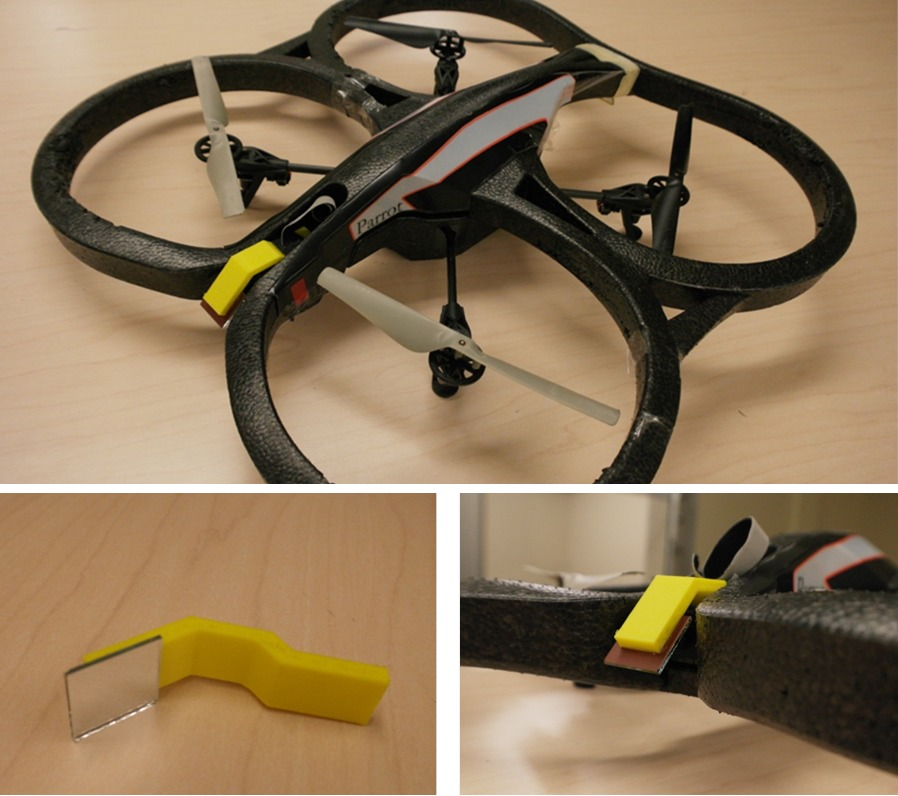
\includegraphics[width=0.489\textwidth, natwidth=901, natheight=861]{figures/chapter2/hw_platform2.jpg}
 \caption{We use the Parrot AR.Drone2.0 as our hardware platform (top), adding a mirror to the front-facing camera in order to detect objects on the ground (bottom).}
 \label{fig:mirror}
\end{figure}

\begin{figure}[t]
 \centering
    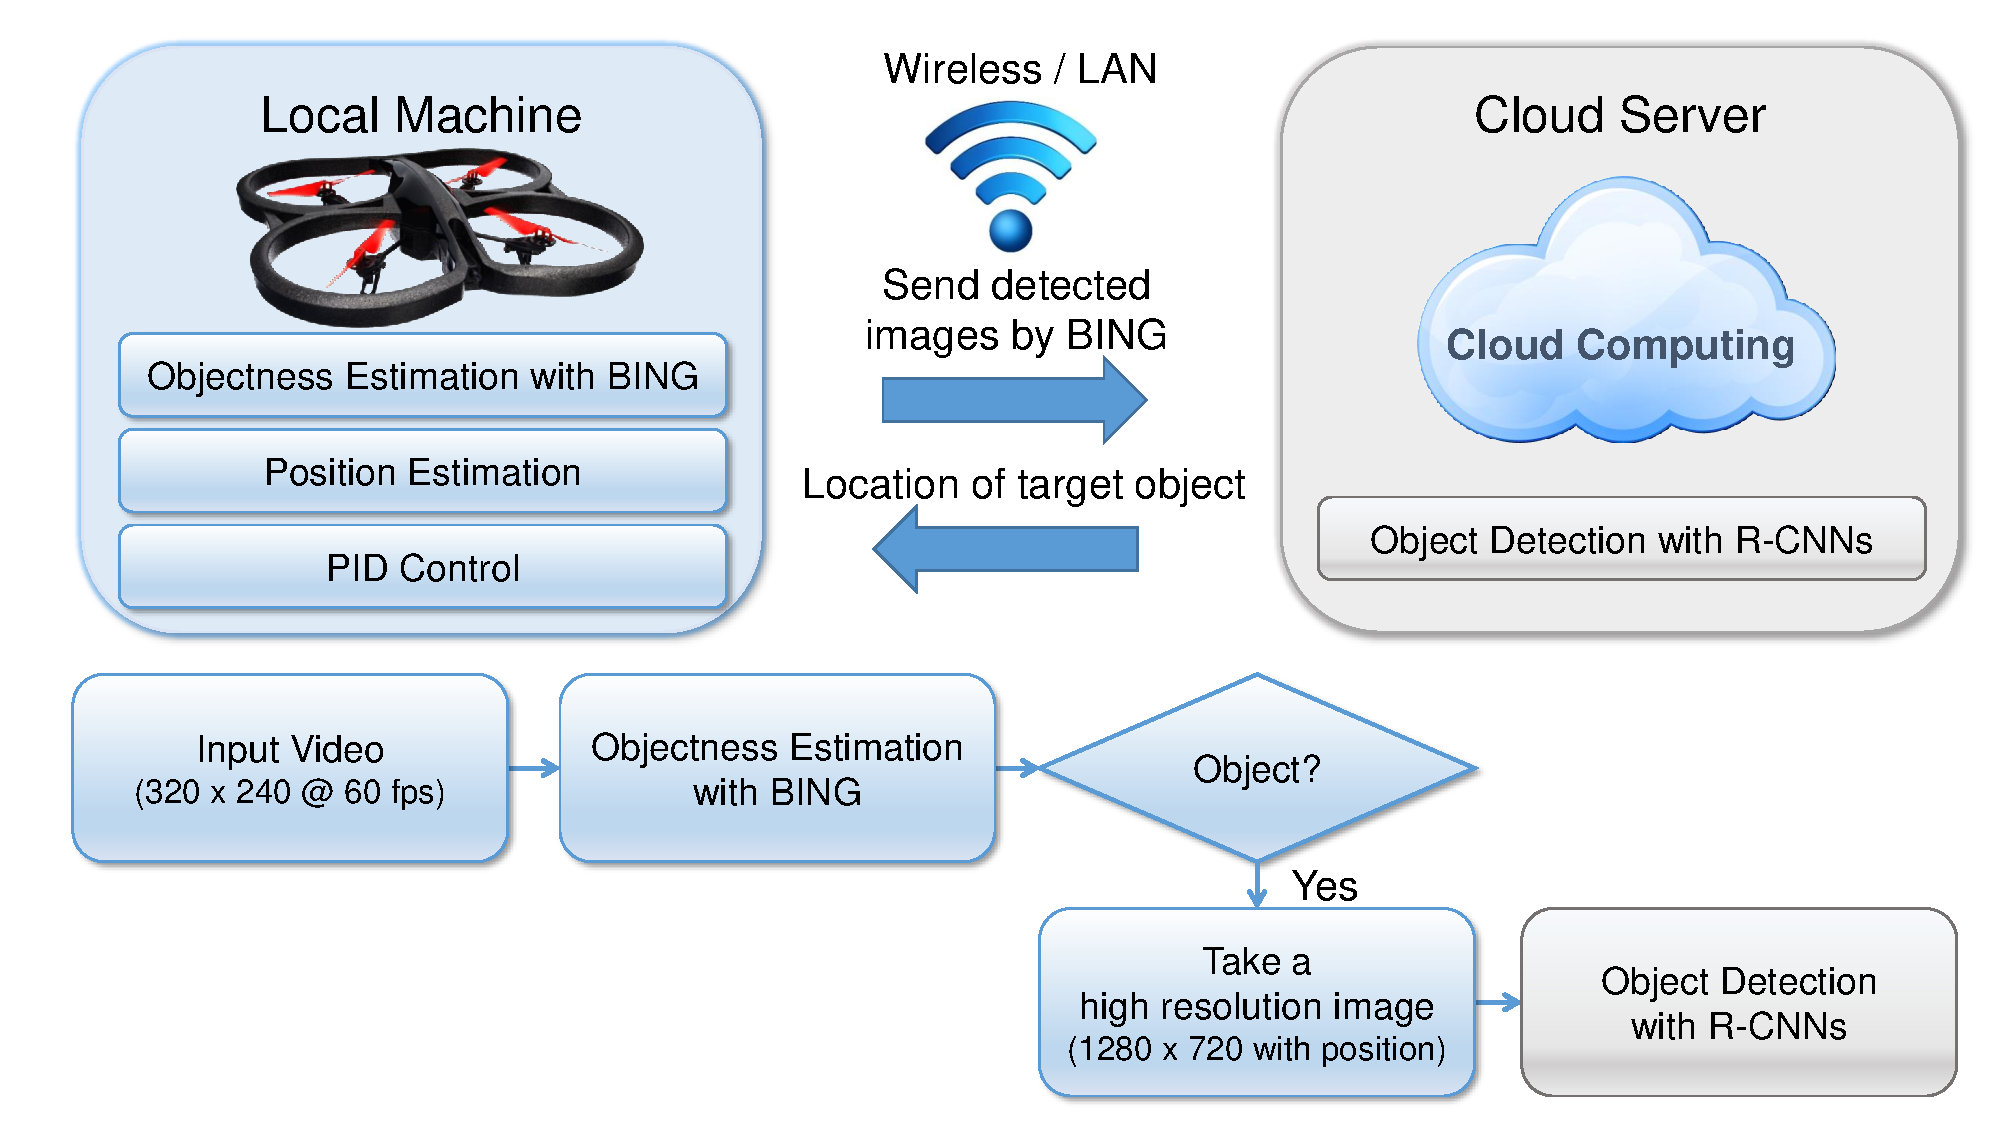
\includegraphics[width=0.489\textwidth]{figures/chapter2/overview.pdf}
 \caption{System Overview: Our approach consists of four main components: BING based objectness estimation, a position estimation for localization, PID control for navigation, and R-CNNs based object detection.
All components are implemented under the ROS framework, so each component can communicate with every other via the ROS network protocol (top). Given input video, the local machine detects generic objects in every frame with BING,
then takes a high resolution image and sends it to the cloud server if the frame contains generic objects. The cloud server then runs R-CNNs based object detection to find a target object (bottom).}
 \label{fig:overview}
\end{figure}

\section{Experimentsal Results}
We conducted three sets of experiments to demonstrate that our approach performs successfully in a realistic but controlled environment. 
In the first set of experiments, we focus on testing the accuracy of recent deep network based object detectors with aerial images taken by the drone.
Secondly, we evaluate the speed of our cloud based object detection approach, comparing with running time of the fastest deep learning based object detector on a local laptop. Finally, we verify our approach with the scenario of a drone searching for a target object in an indoor environment, as a simple simulation of a search-and-rescue or surveillance application. 
The first two sets of experiments were conducted on our aerial image dataset and the last experiment was conducted in an indoor room of about $3m \times 3m$.

\subsection{Object Detection Accuracy}
We first compared the ability of Faster R-CNNs with two recent state-of-the-art object detectors(YOLO ~\cite{yolo}
 and SSD ~\cite{ssd}) to recognize aerial images taken by the drone.
YOLO and SSD are approaches that achieving real-time performance (faster than 30 FPS) on GPU by eliminating the most computationally demanding part(generating region proposals and computing CNN features for each region). 

%To make a fair comparison, we use models that are all pre-trained on the same dataset(Pascal VOC 2007 and Pascal VOC 2012). 
We collected 294 aerial images of 20 object classes and annotated 578 objects in the images. 
These images have the same object classes as the Pascal VOC 2007 dataset and are collected from two sources (some of them are taken by ourselves and the others are collected from 31 publicly available Youtube videos taken by the same drone as ours).
Table ~\ref{tab:accuracy} shows average precision of each algorithm on htis dataset. Here the SSD300 model and SSD500 model have the same architecture and the only difference is the input image size($300 \times 300$ pixels vs. $500 \times 500$ pixels). YOLO and Fast YOLO also use similar architectures except Fast YOLO uses fewer convolutional layers (24 convolutional layers vs. 9 convolutional layers for Fast YOLO).

According to our experiment, Faster R-CNN achieved $83.9\%$ mean average precision (mAP) compared to YOLO models ($78.3\%$ and $79.4\%$) and two SSD models ($81.6\%$ and $82.6\%$).

\begin{table*}[th]
 \caption{Object detection results on our aerial images collected by the drone.}
 \label{table:accuracy}
 \begin{adjustbox}{max width=\textwidth}
 \begin{tabular}{ l | *{20}{c} | l }
    Method &     
                 aero & bike & bird & boat & bottle &
                 bus & car & cat & chair & cow &
                 table & dog & horse & mbike & person &
                 plant & sheep & sofa & train & tv & mAP \\[5pt] \hline
    \\
    Fast YOLO & 
                \textbf{87.5} & 84.6 & 0.0 & 50.0 & 65.5 &
                \textbf{100.0} & 87.9 & 80.0 & \textbf{92.3} & 47.1 &
                60.0 & 75.0 & 88.9 & \textbf{100.0} & 76.6 & \textbf{100.0} &
                54.5 & \textbf{100.0} & 66.7 & 84.6 & 78.3 \\[5pt]
    YOLO &      
                60.9 & 88.2 & 80.0 & 80.0 & 92.3 &
                \textbf{100.0} & 87.2 & \textbf{100.0} & 70.4 & 50.0 &
                40.0 & \textbf{81.0} & 77.8 & 93.4 & 88.7 &
                \textbf{100.0} & 45.2 & \textbf{100.0} & 81.8 & 79.2 & 79.4 \\[5pt]
    SSD300 &    
                60.0 & \textbf{94.1} & 20.0 & \textbf{100.0} & 90.0 &
                \textbf{100.0} & \textbf{100.0} & \textbf{100.0} & 75.0 & 47.8 &
                50.0 & 66.7 & 81.3 & 92.9 & \textbf{92.9} &
                \textbf{100.0} & 66.7 & \textbf{100.0} & 85.7 & 82.6 & 81.6 \\[5pt]
    SSD500 &    
                66.7 & 88.2 & 50.0 & 88.9 & \textbf{100.0} &
                92.9 & 93.2 & \textbf{100.0} & 72.1 & \textbf{65} &
                \textbf{85.7} & 69.6 & 88.9 & 93.8 & 81.7 &
                \textbf{100.0} & 66.7 & 89.5 & 66.7 & \textbf{100.0} & 82.6 \\[5pt]
    Faster R-CNN & 
                70.6 & 93.8 & \textbf{83.3} & 85.7 & 91.9 &
                92.9 & 89.7 & \textbf{100.0} & 87.2 & 62.5 &
                - & 77.3 & \textbf{100.0} & 93.8 & 81.7 &
                66.7 & \textbf{72.7} & \textbf{100.0} & \textbf{100.0} & 62.5 & \textbf{83.9} \\[5pt]
 \end{tabular}
 \end{adjustbox}
\end{table*}

\subsection{Recognition Speed on Cloud System}
Our second set of experiments evaluate the running time performance of the CNN-based object recognition testing the extent to which cloud computing could improve recognition times, and the variability of the unpredictable communication times. We use the same dataset as in the previous section and compare the speed of each algorithm using GPU on a simulated cloud machine.
We measure the running time including image loading, pre-processing, and output parsing (post-processing) time.

Fig. ~\ref{fig:compare_algorithm} shows the running time of each algorithm as a function of its accuracy. 
The result shows detection speed and accuracy are inverse related. Fast YOLO showed te highest speed (57.4 FPS) with the lowest accuracy (mAP $78.3\%$), while Faster R-CNN has the lowest speed (3.48 FPS) with the highest accuracy (mAP $83.9\%$).

Then we compare Fast YOLO on a local laptop versus Faster R-CNN on the simulated cloud. 
A comparison of these computing facilities are showed in Table ~\ref{tab:hw}. 
Fig. ~\ref{fig:bar_plot} shows the average running time of Fast YOLO on local machine is $7.31$ seconds per image while for Faster R-CNN running on remote cloud is $1.29$ seconds including latencies for sending each image to the cloud (which averaged about 600 ms) and for exchanging detected results and other command messages (which averaged 0.41 ms). Thus the cloud-based recognition performed about 5.7 times faster than the local Fast YOLO on average.

\begin{figure}[t]
\begin{center}
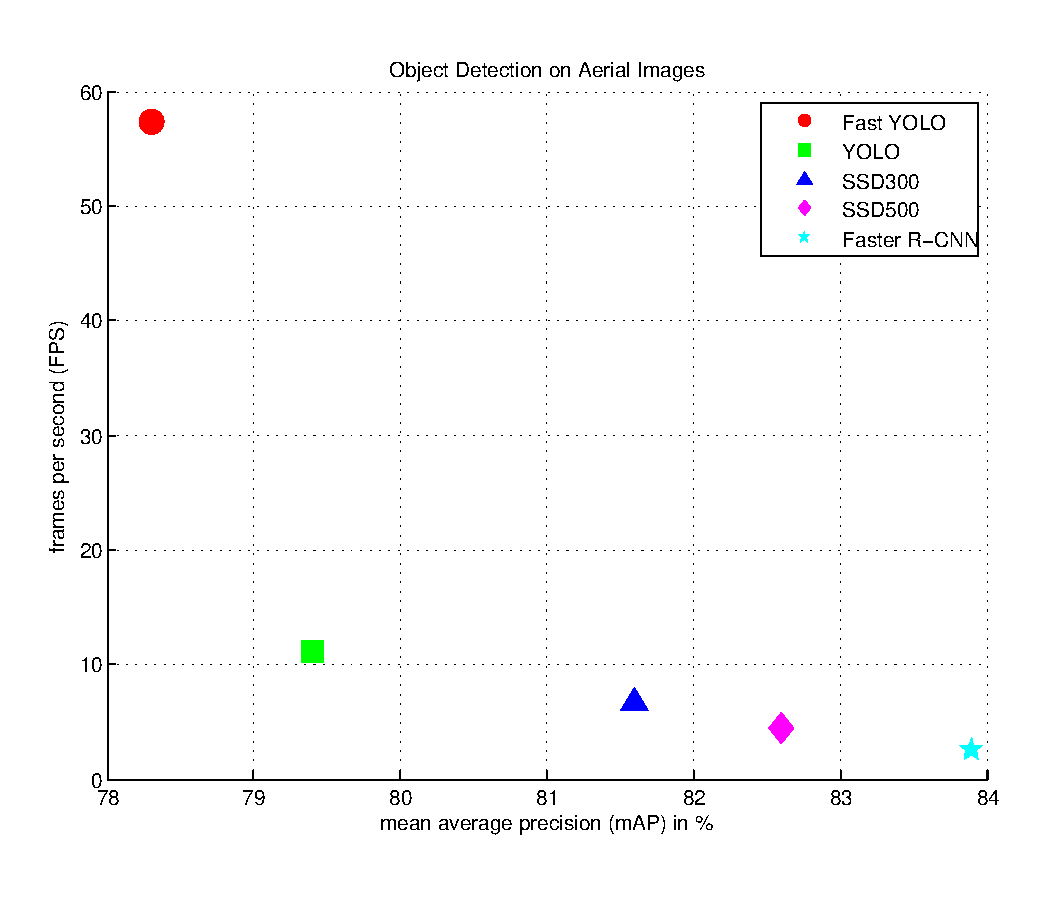
\includegraphics[width=0.489\textwidth]{figures/chapter2/drone_comparing_algorithms.pdf}
\end{center}
\caption{A running time comparison of recent state-of-the-art object detectors on our aerial images.}
\label{fig:compare_algorithm}
\end{figure}

\begin{figure}[t]
\begin{center}
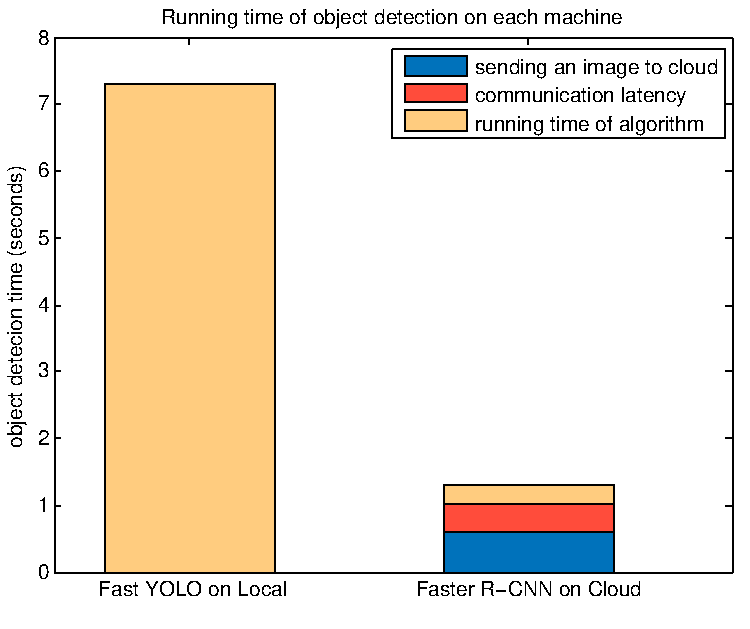
\includegraphics[width=0.489\textwidth]{figures/chapter2/drone_running_time.pdf}
\end{center}
\caption{Running time of object detection on each machine.}
\label{fig:bar_plot}
\end{figure}

\begin{table}[b]
 \caption{Hardware Comparison between Local and Cloud Machine}
 \label{table:hw}
 \begin{center}
  \begin{tabular}{ l m{3cm} m{3cm} }
   \hline
    & local computer  & cloud computer \\
   \hline
   CPUs & one Intel Core \newline i7-4700HQ @ 2.4GHz & two Intel Xeon \newline E5-2680 v3 @ 2.5GHz \\ \hline
   GPUs & one Nvidia \newline GeForce GTX 770M & two Nvidia Tesla K40 \\ \hline
   RAM & 16 GB & 128 GB \\ \hline
%   GPUs Use & no  & yes \\
  \end{tabular}
 \end{center}
\end{table}

\subsection{Target Search with a Drone}
In the test scenario, we use a screwdriver as a target object and scattered various distractor objects on the floor in the indoor test room. 
The drone started this object searching mission with lower-resolution downward-facing camera, and run the BING algorithm for finding generic objects given the input video.
Fig. ~\ref{fig:searching} shows a sequence of images taken during this test. When the drone finds any ``interesting'' objects on the floor, it switches to the front-facing camera to capture a photo at a higher resolution, then take picture of the candidate area and sends it to the cloud system ($t=3$s and $t=8$s).
After this, the drone switch the camera back to the downward-facing camera and proceeds to the other candidate positions. 
The cloud system performs recognition in the meantime.
The drone performs the same steps until it finds a target object, at which point the mission is completed ($t=17$s).

\begin{figure*}[th]
\centering
\begin{tabular}{@{}c@{\,\,\,}c@{\,\,\,}c@{\,\,\,}c@{\,\,\,}c@{\,\,\,}}
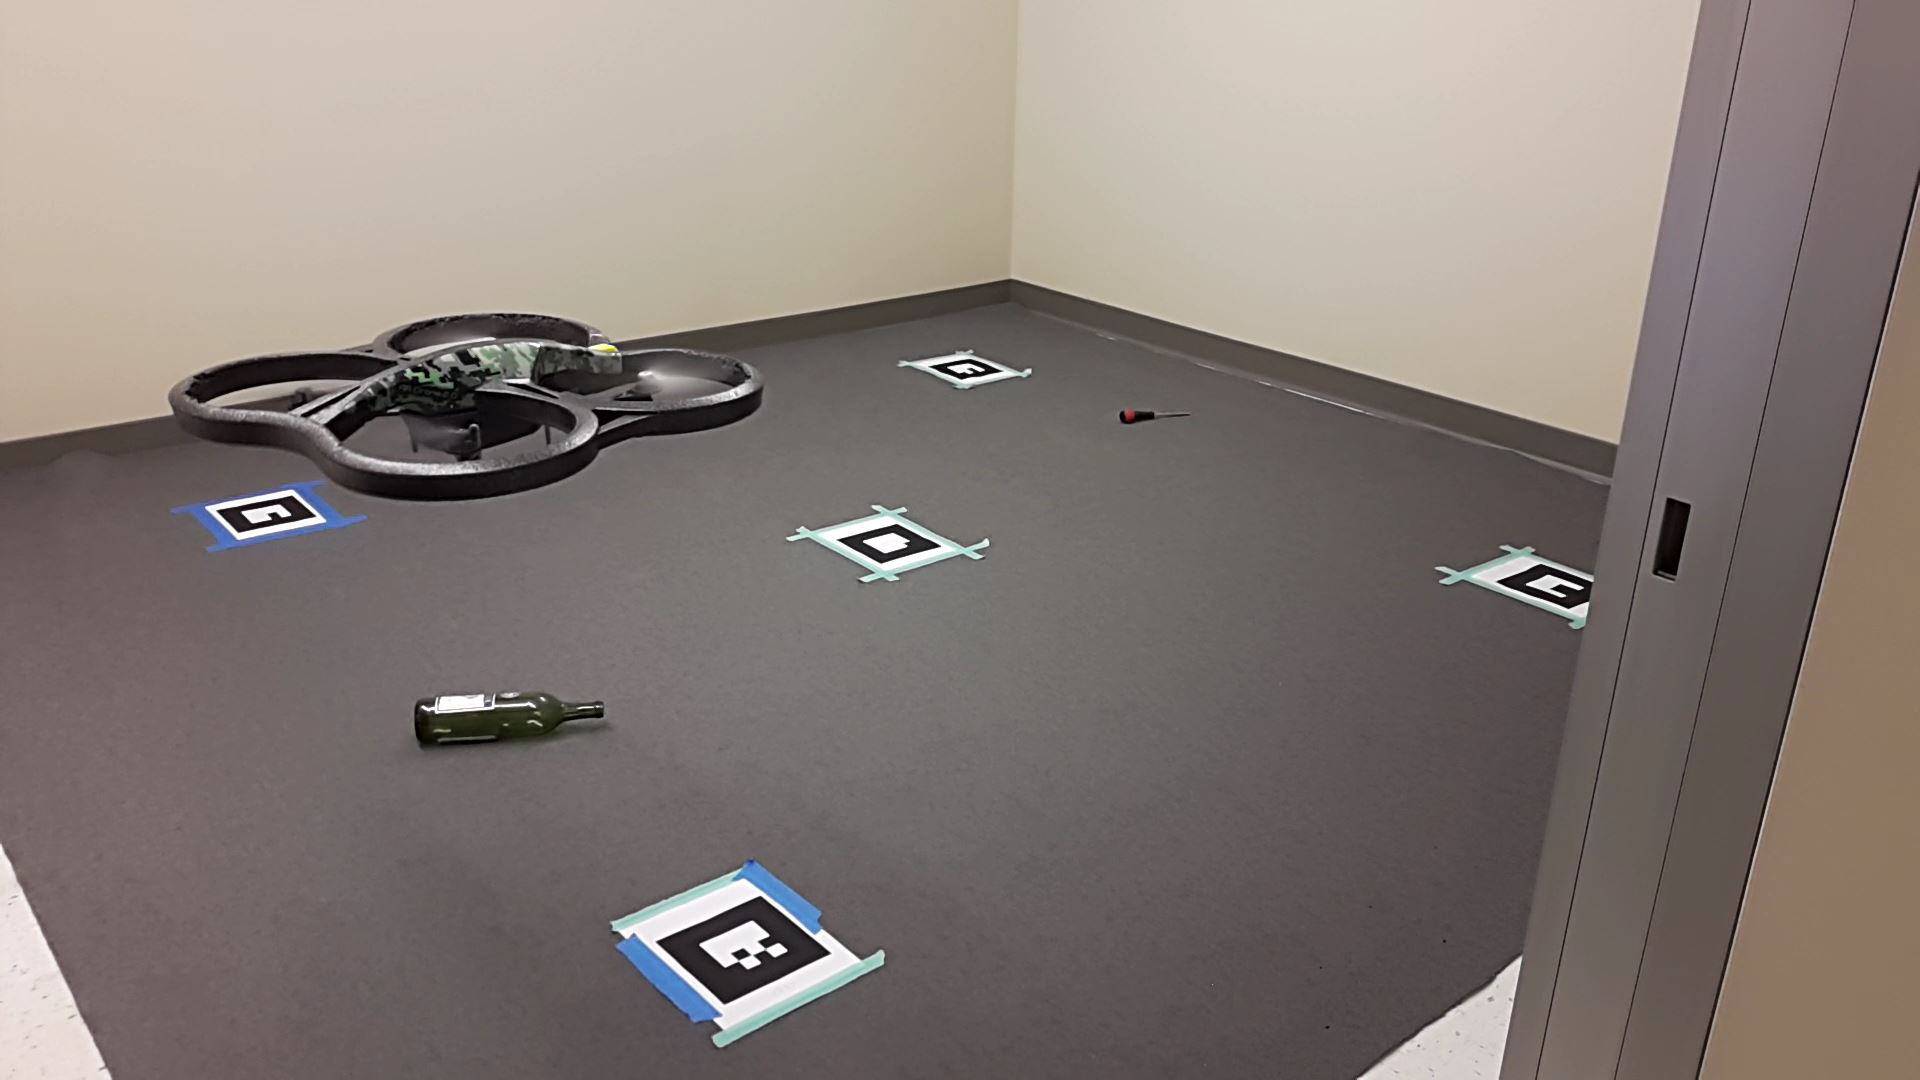
\includegraphics[width=0.2\textwidth]{figures/chapter2/search_t0.jpg} &
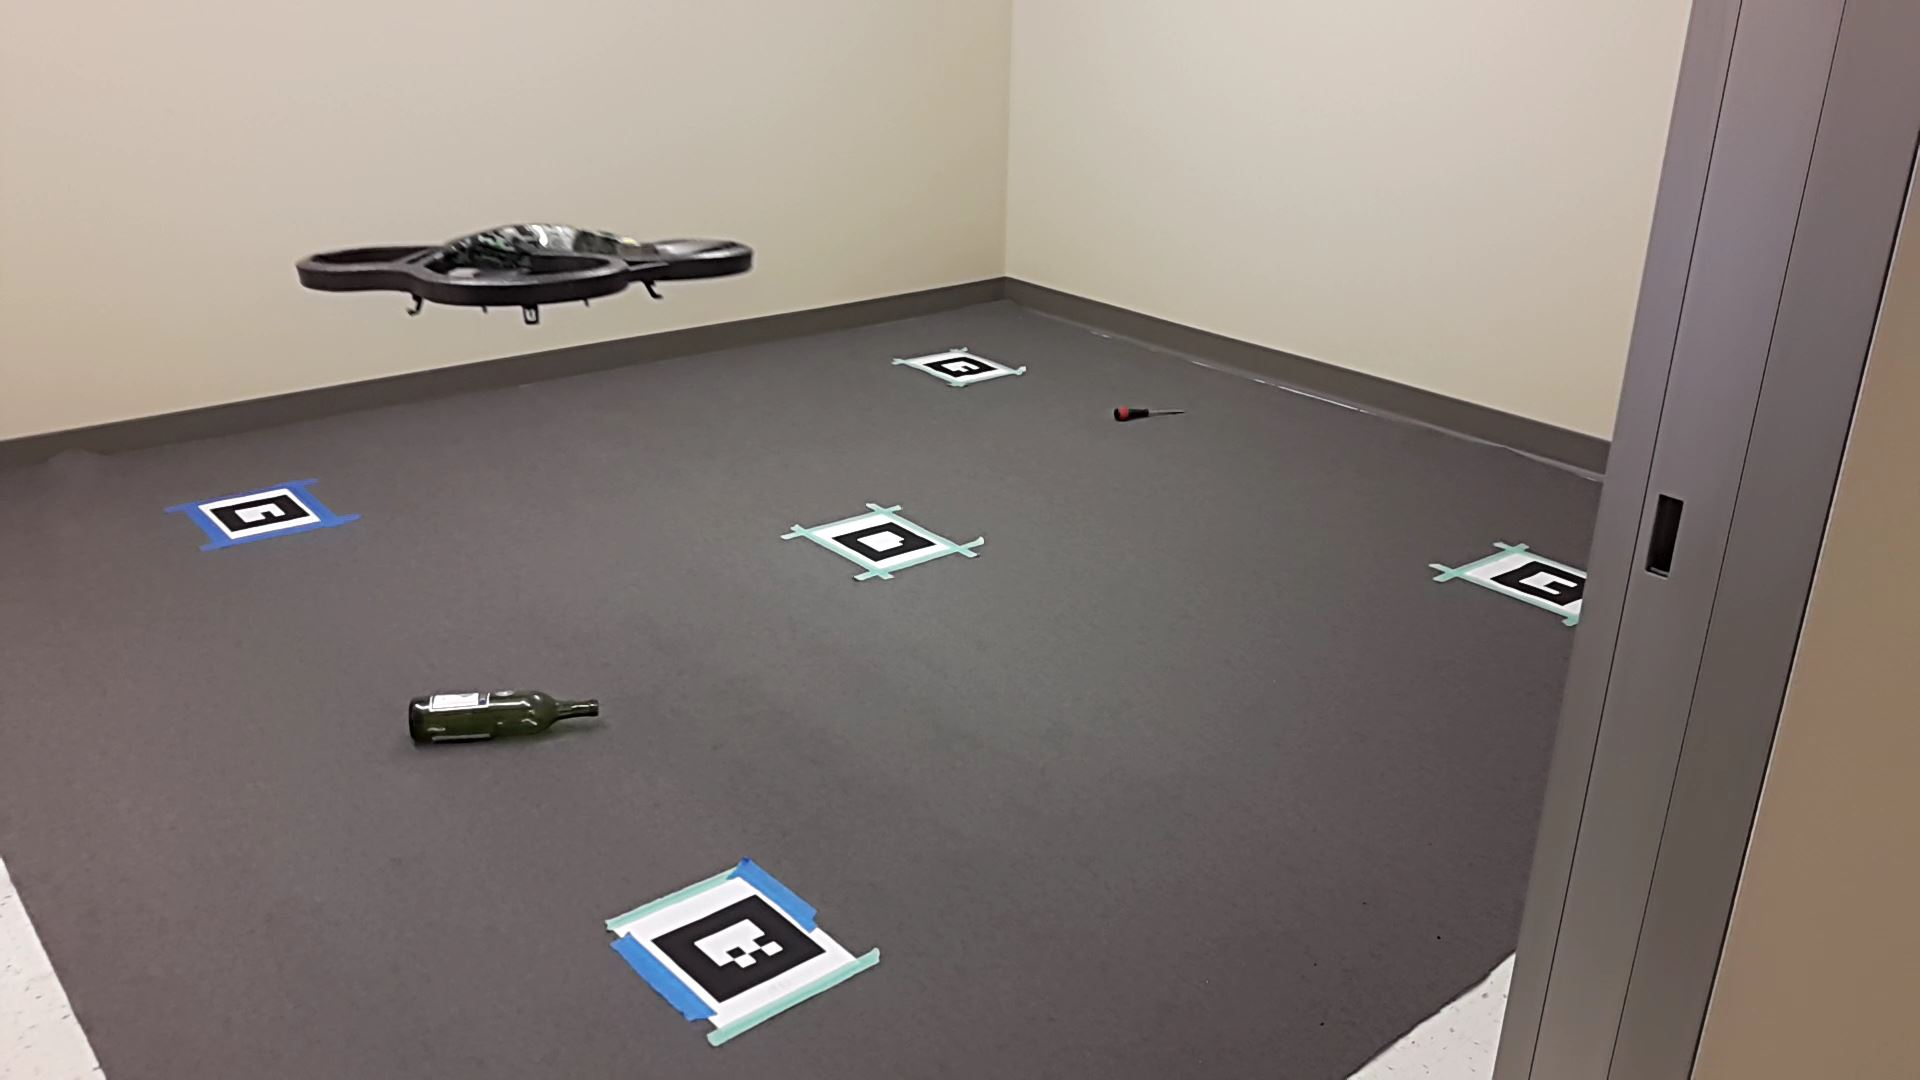
\includegraphics[width=0.2\textwidth]{figures/chapter2/search_t3.jpg} &
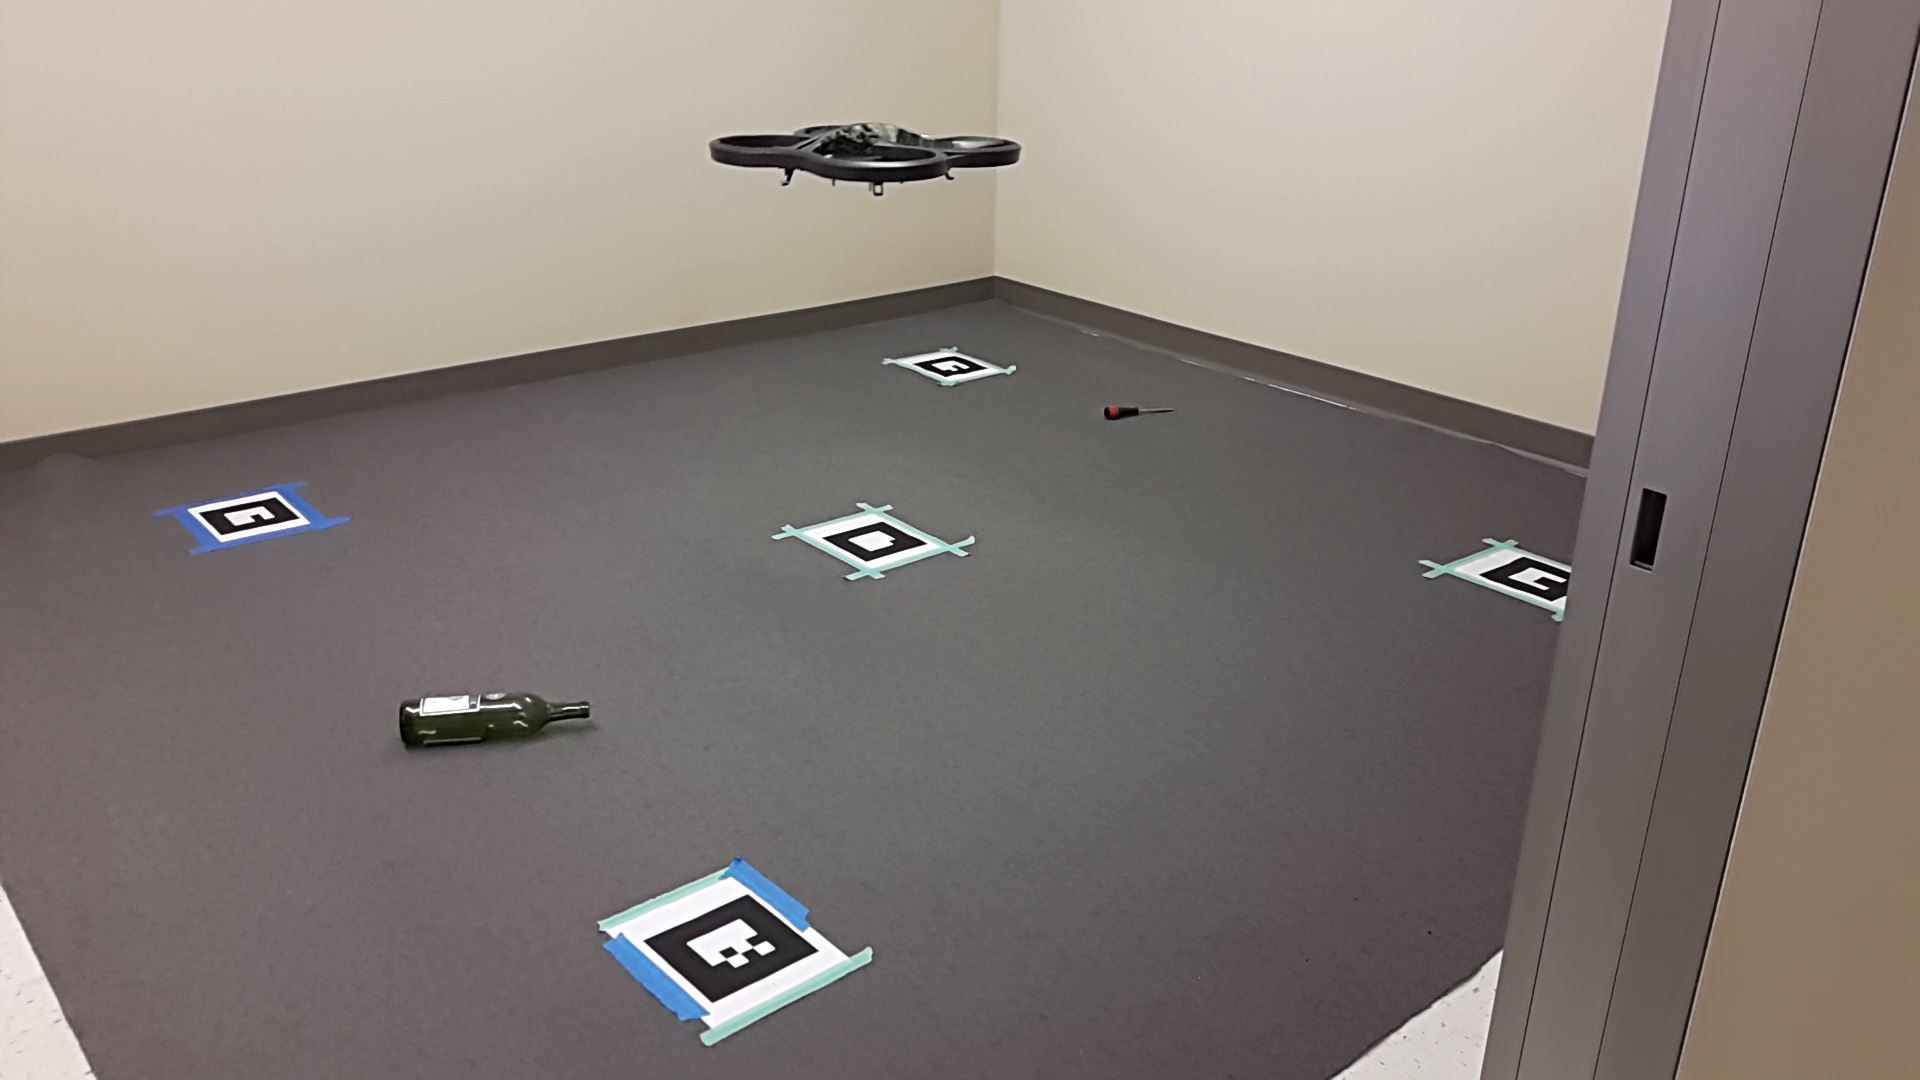
\includegraphics[width=0.2\textwidth]{figures/chapter2/search_t8.jpg} &
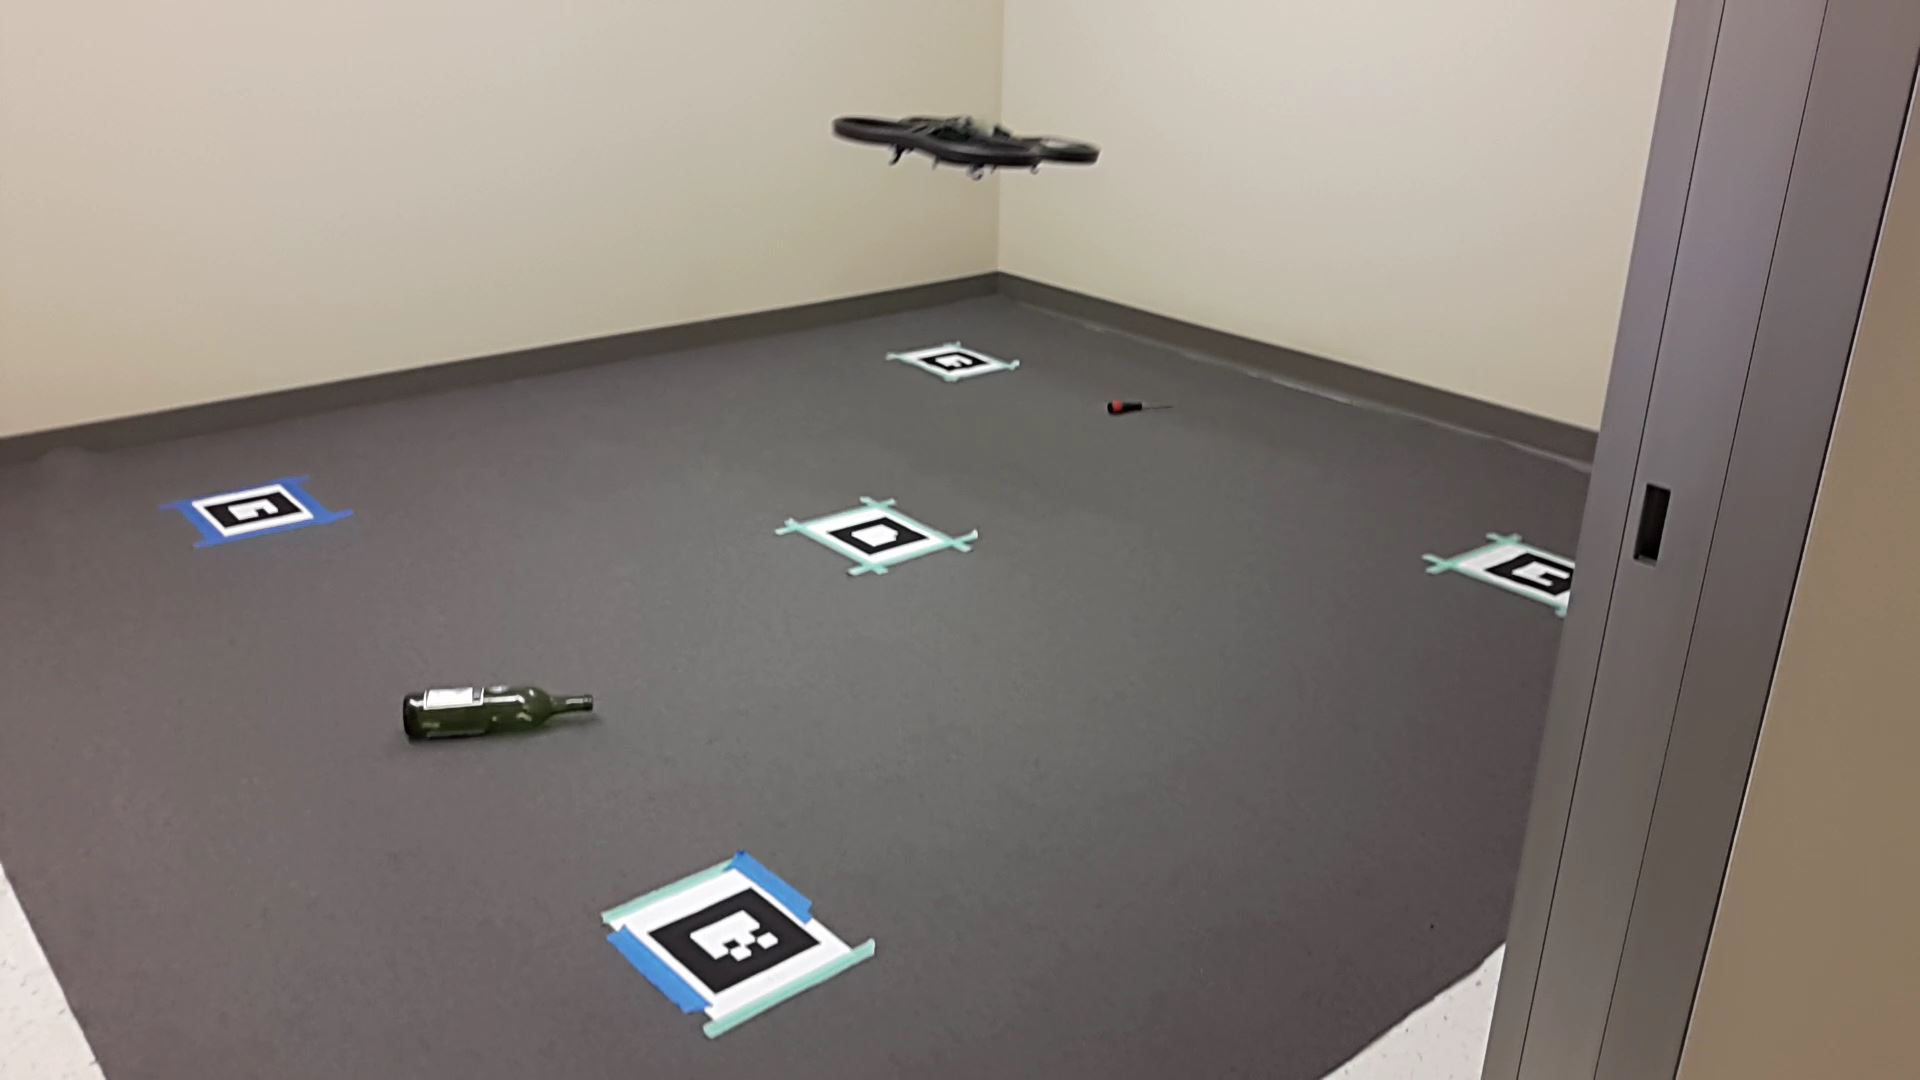
\includegraphics[width=0.2\textwidth]{figures/chapter2/search_t13.jpg} &
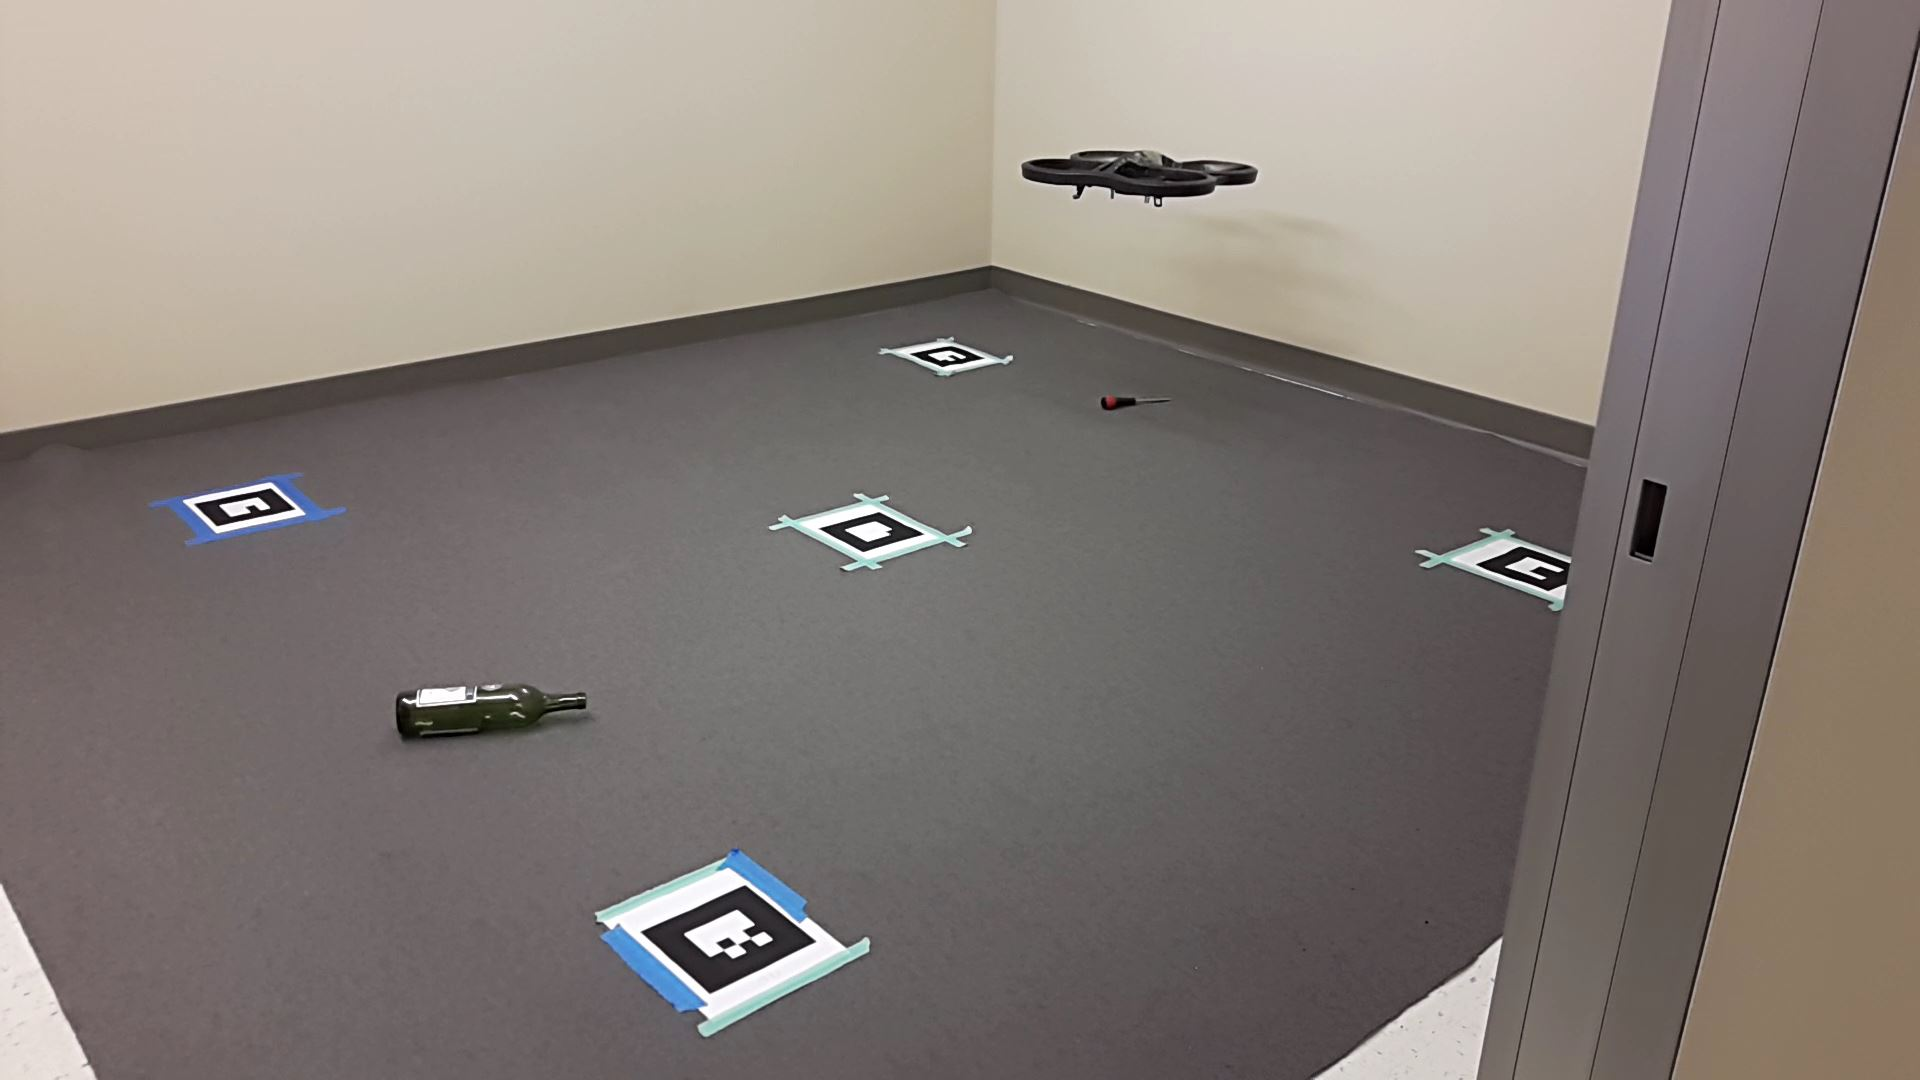
\includegraphics[width=0.2\textwidth]{figures/chapter2/search_t17} \\
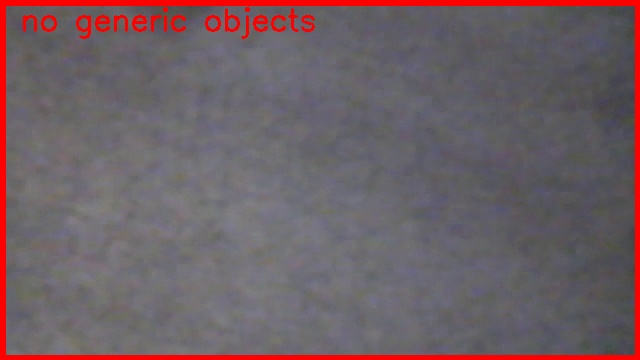
\includegraphics[width=0.2\textwidth]{figures/chapter2/bing_t0.jpg} &
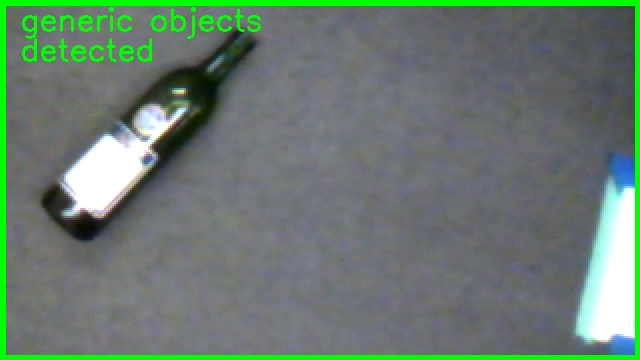
\includegraphics[width=0.2\textwidth]{figures/chapter2/bing_t3.jpg} &
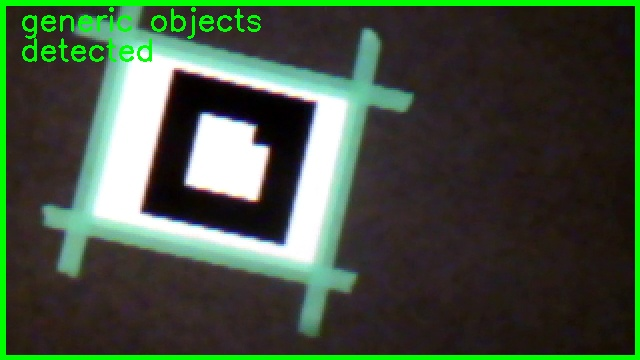
\includegraphics[width=0.2\textwidth]{figures/chapter2/bing_t8.jpg} &
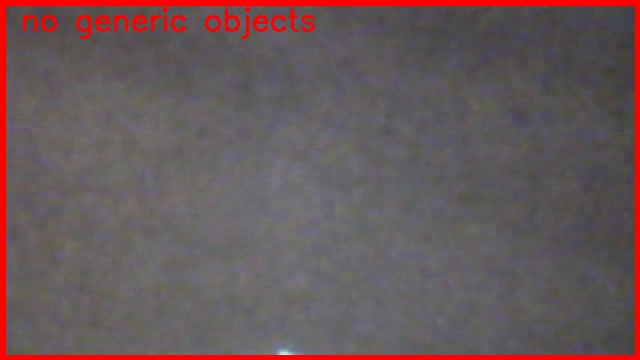
\includegraphics[width=0.2\textwidth]{figures/chapter2/bing_t13.jpg} &
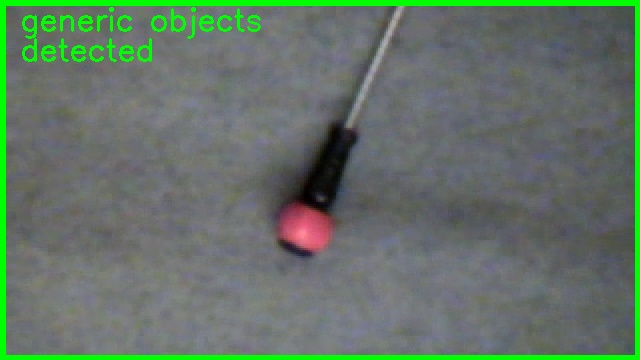
\includegraphics[width=0.2\textwidth]{figures/chapter2/bing_t17} \\
\textit{t} = 0 s &
\textit{t} = 3 s &
\textit{t} = 8 s &
\textit{t} = 13 s&
\textit{t} = 17 s\\
&
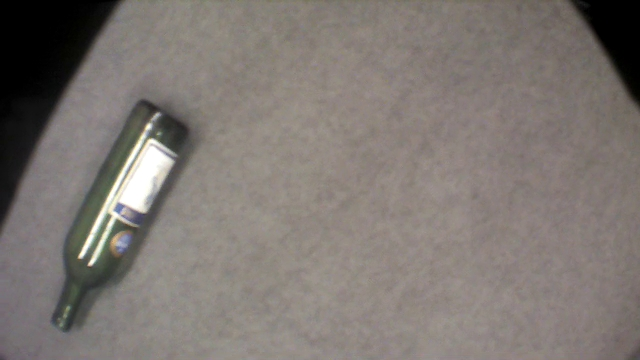
\includegraphics[width=0.2\textwidth]{figures/chapter2/front_t3} &
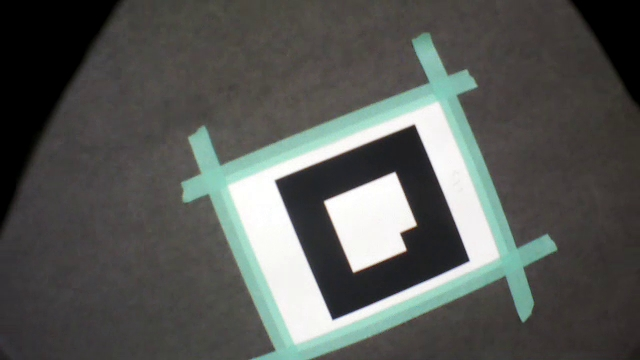
\includegraphics[width=0.2\textwidth]{figures/chapter2/front_t8} &
&
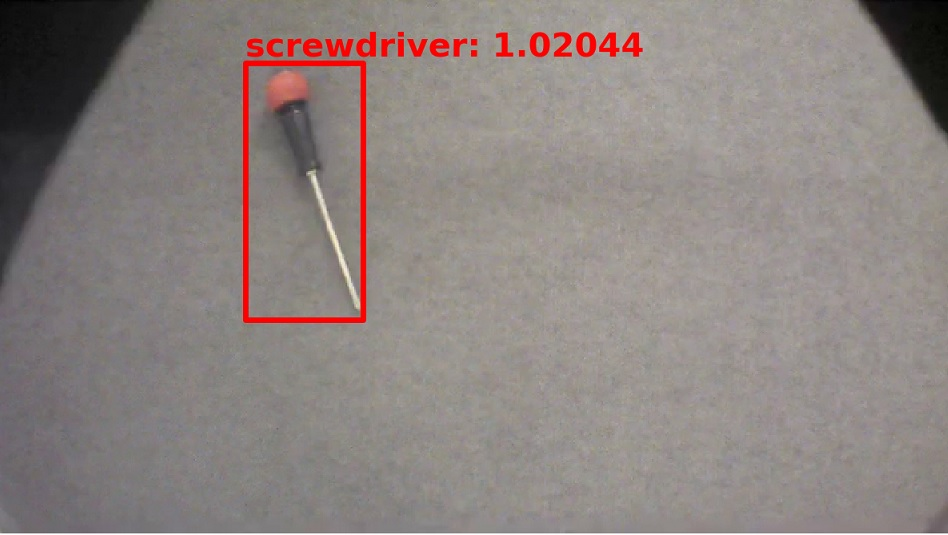
\includegraphics[width=0.2\textwidth]{figures/chapter2/rcnn_result_t17.jpg} \\
\end{tabular}
\caption{Target Search with a Drone: First rows show movements of the drone during the experiment,
and second and third rows indicate detection results from BING and R-CNNs respectively.
At \textit{t} = 0 s the drone started to search for a target object and did not find generic objects with BING.
At \textit{t} = 3 s, \textit{t} = 8 s, the drone found generic objects with BING, thus took high resolution pictures and sent them to cloud server.
However, R-CNNs did not detect a target object in those images.
At \textit{t} = 17 s, the drone found generic objects again, thus it took the high resolution picture and sent it to cloud server.
Then, finally R-CNNs based object detector found a target object.}
\label{fig:searching}
\end{figure*}
